% =============================================================================
% VERSIÓN RBEF — Revista Brasileira de Ensino de Física (sección Artigos Gerais)
% Protocolo RBEF: .tex UTF-8, sin TikZ, \bibitem, título/resumen/palabras
% clave bilingües (español + inglés), referencias en orden de citación,
% ecuaciones citadas como "ecuación (n)".
% Compilar: pdflatex borrador_rbef.tex  (dos pasadas)
% =============================================================================

% Layout tipo RBEF publicada: cabecera y resúmenes a ancho completo,
% cuerpo a dos columnas (los fascículos recientes de la revista usan
% este formato; el protocolo no exige columnas para la submissão).
\documentclass[10pt,a4paper,twocolumn]{article}

\usepackage[utf8]{inputenc}
\usepackage[T1]{fontenc}
\usepackage[spanish,es-nodecimaldot]{babel}
\usepackage{amsmath,amssymb}
\usepackage{graphicx}
\usepackage{booktabs}
\usepackage[margin=2cm]{geometry}
\usepackage[colorlinks=true,linkcolor=blue,citecolor=blue,urlcolor=blue]{hyperref}

\newcommand{\eps}{\varepsilon}
\newcommand{\gstar}{g^*}
\newcommand{\lammps}{\textsc{Lammps}}

\begin{document}

% --- Cabecera y resúmenes a ancho completo -------------------------------------
\twocolumn[{%
\begin{center}
    {\LARGE\bfseries ¿A dónde se va la energía de una pelota que rebota?\\
    Partición energética del impacto de nanocúmulos de Lennard-Jones\\
    mediante dinámica molecular\par}
    \vspace{6pt}
    {\large\itshape Where does the energy of a bouncing ball go?
    Energy partition in the\\ impact of Lennard-Jones nanoclusters via
    molecular dynamics\par}
    \vspace{12pt}
    Felipe Wasaff$^{1,*}$ \quad y \quad Gonzalo Gutiérrez$^{2}$\\[4pt]
    {\small $^{1}$Instituto de Matemáticas, Pontificia Universidad
    Católica de Valparaíso, Valparaíso, Chile}\\
    {\small $^{2}$Departamento de Física, Facultad de Ciencias,
    Universidad de Chile, Santiago, Chile}\\[2pt]
    {\small $^{*}$Autor de correspondencia: felipe.wasaff.g@mail.pucv.cl
    --- ORCID: \href{https://orcid.org/0009-0006-0280-4215}%
    {0009-0006-0280-4215}}\\[4pt]
    {\small \today}
\end{center}
\vspace{8pt}
\begin{quotation}
\small
\noindent
En los cursos de mecánica, el coeficiente de restitución $e<1$ resume toda
la física del rebote inelástico en un número, y la energía ``perdida'' se
atribuye genéricamente a fricción, calor o sonido. En este trabajo abrimos
esa caja negra con un experimento computacional accesible: la caída y el
rebote de un nanocúmulo de Lennard-Jones de $N$ átomos sobre una superficie
cristalina, simulados con el programa abierto \lammps{} en un computador
personal. Midiendo la energía en el primer apogeo identificamos cuatro
canales cuya suma es exactamente la energía de impacto $E_0$: la energía
recuperada por el centro de masa ($\alpha_{\rm cm}=e_1^2$), el
calentamiento vibracional interno de la bola ($\alpha_{T_B}\approx0.22$),
la expansión anarmónica de la bola ($\alpha_{\Delta V_B}\approx0.2$--$0.3$)
y los fonones de la superficie ($\alpha_{\rm surf}\approx0.07$--$0.16$).
La mayor parte de la energía no recuperada queda
\emph{dentro de la propia pelota}, no en el piso. Promediando sobre las
orientaciones del cúmulo y midiendo el número de átomos de superficie
activados, mostramos que la superficie es un reservorio ancho pero
casi elástico: la fracción de la energía \emph{disipada} que queda en la
bola sigue una equipartición entre sus $3N-3$ modos internos y una capacidad
neta pequeña y aproximadamente constante de la superficie
($N_c^{\rm ef}\approx25$), de modo que esa fracción tiende a $1$ ---no a
$1/2$--- para bolas grandes. El sistema conecta en un solo problema la
mecánica newtoniana, la física estadística y los métodos computacionales;
se incluyen los archivos de entrada, los scripts de análisis y actividades
propuestas para el aula.

\medskip
\noindent\textbf{Palabras clave:} dinámica molecular, coeficiente de
restitución, partición de energía, equipartición, nanocúmulos, enseñanza
de física computacional.

\bigskip
\noindent In mechanics courses, the coefficient of restitution $e<1$
summarizes all the physics of an inelastic bounce in a single number, and
the ``lost'' energy is generically attributed to friction, heat or sound.
In this work we open that black box with an accessible computational
experiment: the fall and bounce of a Lennard-Jones nanocluster of $N$
atoms on a crystalline surface, simulated with the open-source code
\lammps{} on a personal computer. Measuring the energy at the first apex
we identify four channels whose sum is exactly the impact energy $E_0$:
the energy recovered by the center of mass ($\alpha_{\rm cm}=e_1^2$), the
internal vibrational heating of the ball ($\alpha_{T_B}\approx0.22$), the
anharmonic expansion of the ball ($\alpha_{\Delta V_B}\approx0.2$--$0.3$)
and the surface phonons ($\alpha_{\rm surf}\approx0.07$--$0.16$). The
result is surprising: most of the non-recovered energy stays \emph{inside
the ball itself}, not in the floor. Averaging over cluster orientations and
directly counting the activated surface atoms, we show that the surface is a
broad but nearly elastic reservoir: the fraction of the \emph{dissipated}
energy retained by the ball follows an equipartition between its $3N-3$
internal modes and a small, roughly constant net surface capacity
($N_c^{\rm ef}\approx25$), so that this fraction tends to $1$ ---not $1/2$---
for large balls. The system connects Newtonian mechanics, statistical physics
and computational methods in a single problem; input files, analysis scripts
and proposed classroom activities are included.

\medskip
\noindent\textbf{Keywords:} molecular dynamics, coefficient of
restitution, energy partition, equipartition, nanoclusters, computational
physics teaching.
\end{quotation}
\vspace{14pt}
}]

% =============================================================================
\section{Introducción}
\label{sec:intro}
% =============================================================================

Una pelota que se suelta desde una altura $h_0$ rebota hasta una altura
$h_1<h_0$. En los cursos de mecánica este hecho se codifica en el
coeficiente de restitución,
\begin{equation}
    e = \frac{|v_{\rm despegue}|}{|v_{\rm impacto}|}, \qquad
    \frac{h_1}{h_0} = e^2 < 1,
    \label{eq:cor}
\end{equation}
y la energía faltante, $(1-e^2)Mgh_0$, se atribuye a ``fricción'',
``calor'' o ``sonido'' sin mayor detalle~\cite{Cross1999,Aguiar2003}.
Esa respuesta, aunque correcta, esconde la pregunta físicamente
interesante: ¿\emph{dónde} queda esa energía inmediatamente después del
rebote? ¿En la pelota o en el piso? ¿Como movimiento térmico o como
deformación? Para una pelota macroscópica el desglose es inaccesible en la
práctica, pero para una pelota \emph{nanométrica} simulada átomo a átomo
la contabilidad energética puede hacerse exacta: la dinámica molecular
(MD) permite medir cada término del hamiltoniano en cada instante
\cite{AllenTildesley,FrenkelSmit}.

Este problema fue propuesto como experimento computacional por Gutiérrez
et al.~\cite{Gutierrez2012}, quienes estudiaron con MD el rebote de un
cúmulo de argón de $N\approx79$ átomos sobre una superficie cristalina
bajo gravedad, con interacción bola--superficie puramente repulsiva. Sus
resultados principales fueron que la secuencia de alturas $h_n$ decae más
rápido que una serie geométrica, que durante la colisión la energía de
contacto almacena transitoriamente la mayor parte de la energía
``disipada'', y que para caídas grandes la bola se funde en el impacto.
Aquel análisis, sin embargo, se concentró en lo que ocurre \emph{durante}
el contacto; no cuantificó cómo queda repartida la energía una vez que la
bola se separa y alcanza su primer apogeo.

En este artículo retomamos y extendemos ese experimento con el programa
abierto \lammps~\cite{Thompson2022}, con tres objetivos pedagógicos:
\textbf{(i)}~mostrar que con herramientas gratuitas y un computador
personal (cada simulación toma $\sim$1--2 minutos) un estudiante puede
responder cuantitativamente la pregunta ``¿a dónde se va la energía?'',
descomponiéndola en \emph{cuatro canales} que suman exactamente $E_0$;
\textbf{(ii)}~conectar ese resultado con la física estadística: un
argumento de equipartición predice cómo la fracción absorbida escala con
el número de átomos $N$, y el barrido $N\in\{1,2,7,13,55,79,87\}$ lo
verifica; \textbf{(iii)}~ilustrar buenas prácticas de la simulación
computacional ---conservación de energía, reproducibilidad, análisis de
convenciones de medición--- que rara vez se discuten en textos
introductorios. Todos los archivos de entrada y scripts de análisis están
disponibles en un repositorio público (Sección~\ref{sec:metodos}).

% =============================================================================
\section{El sistema: una pelota de \texorpdfstring{$N$}{N} átomos}
\label{sec:modelo}
% =============================================================================

Trabajamos en unidades reducidas de Lennard-Jones (LJ): las longitudes se
miden en $\sigma$, las energías en $\eps$ y el tiempo en
$\tau=\sqrt{m\sigma^2/\eps}$. Para el argón, $\sigma\approx3.4$~\AA,
$\eps\approx0.0104$~eV y $\tau\approx2.15$~ps, de modo que todo el
experimento ocurre en decenas de nanosegundos y en una caja de pocos
nanómetros: es la versión nanométrica de la pelota que rebota.

Todos los pares de átomos interactúan mediante el potencial LJ
\begin{equation}
    U_{\mathrm{LJ}}(r) = 4\eps \left[ \left(\frac{\sigma}{r}\right)^{12}
    - c_{ij}\left(\frac{\sigma}{r}\right)^{6} \right],
    \quad r < r_c = 2.5\,\sigma,
    \label{eq:lj}
\end{equation}
con $c_{ij}=1$ (atracción y repulsión) para pares bola--bola y
superficie--superficie. Para el par bola--superficie consideramos dos
casos: $c_{ps}=0$ (rebote puro, sin adhesión, el caso
de~\cite{Gutierrez2012}) y $c_{ps}=1$ (con adhesión,
Sección~\ref{sec:adhesion}).

La ``pelota'' es un cúmulo FCC de $N$ átomos construido con las capas
esféricas completas de la red ($N=1, 13, 55, 79, 87,\ldots$), minimizado
en vacío antes de soltarlo; agregamos $N=2$ y $7$ como controles del
régimen molecular. El ``piso'' es una losa FCC de $8\times8\times6$ celdas
($N_s\approx1540$ átomos) con las dos capas inferiores fijas y condiciones
periódicas laterales. La gravedad reducida $\gstar=0.026\,\sigma/\tau^2$
actúa solo sobre la bola, que se suelta desde el reposo a una altura
$h_0$. No hay termostato: la dinámica es puramente newtoniana (NVE) y la
temperatura inicial es $T=0$, así que \emph{toda} la energía del problema
proviene de la caída.

La contabilidad energética se organiza en cuatro términos, medidos en el
primer apogeo (cuando la bola, ya separada, alcanza su altura máxima
$h_1$) y normalizados por la energía de impacto $E_0=Mg\,h_0^{\rm ef}$:
\begin{align}
    \alpha_{\rm cm}     &= \frac{h_1}{h_0^{\rm ef}} = e_1^2
        &&\text{(energía recuperada por el CM),} \label{eq:acm}\\
    \alpha_{T_B}        &= \frac{T_B^{(1)}}{E_0}
        &&\text{(KE vibracional interna de la bola),} \label{eq:atb}\\
    \alpha_{\rm surf}   &= \frac{\Delta(K_S + V_{\rm surf})}{E_0}
        &&\text{(fonones de la superficie),} \label{eq:asurf}\\
    \alpha_{\Delta V_B} &= \frac{V_B^{(1)}-V_B^{(0)}}{E_0}
        &&\text{(expansión anarmónica de la bola),} \label{eq:avb}
\end{align}
donde $h_0^{\rm ef}$ es la altura de caída medida desde el nivel de
contacto, $T_B$ es la energía cinética de los átomos de la bola
\emph{descontado} el movimiento del centro de masa, y $V_B$ es la energía
potencial interna de la bola. La conservación de la energía garantiza
$\alpha_{\rm cm}+\alpha_{T_B}+\alpha_{\Delta V_B}+\alpha_{\rm surf}=1$, y
esa suma, medida de forma independiente canal por canal, es el primer
control de calidad de la simulación (Sección~\ref{sec:metodos}).

% =============================================================================
\section{La simulación con LAMMPS}
\label{sec:metodos}
% =============================================================================

\lammps{}~\cite{Thompson2022} es un programa de dinámica molecular
gratuito y de código abierto, disponible en los repositorios de las
distribuciones de Linux habituales. Nuestro archivo de entrada
(\texttt{in.bounce\_cluster}) tiene unas 150 líneas comentadas y expone
como variables externas la altura $h_0$, el tamaño del cúmulo, la gravedad
y el interruptor de adhesión $c_{ps}$, de modo que el barrido completo de
este artículo se corre con un lazo de shell. En un computador portátil
(un solo núcleo, $\sim1.4\times10^6$ átomos$\cdot$paso/s) cada rebote de
$400\,\tau$ toma alrededor de 1.5 minutos. Los archivos de entrada, los
cúmulos pre-minimizados y los scripts de análisis en Python (numpy +
matplotlib + scipy) están disponibles en
\url{https://github.com/fwasaff/inelastic-rebound-md}.

Tres detalles técnicos merecen discutirse porque son, en sí mismos,
lecciones de simulación:

\textbf{(a) Cúmulos de tamaño exacto.} Crear la bola recortando una esfera
de una red (\texttt{create\_atoms region sphere}) produce un número de
átomos que depende de dónde caiga el centro de la esfera (79--84 átomos
para radio $2.64\,\sigma$). Construir el cúmulo por capas esféricas
completas y minimizarlo antes de soltarlo garantiza el mismo $N$ en todas
las corridas y una bola inicialmente fría, sin energía interna residual
que contamine la medición de $\alpha_{T_B}$.

\textbf{(b) Conservación de energía y potencial desplazado.} Con el
potencial de la ecuación~(\ref{eq:lj}) truncado en $r_c$ \emph{sin
desplazar}, cada par de átomos que cruza $r_c$ introduce un salto de
$\pm|U(r_c)|=0.016\,\eps$ en la energía potencial registrada; el error
acumulado alcanza 2--6\% de $E_0$ por impacto y arruina la contabilidad de
los canales. Truncando \emph{y desplazando} el potencial
(\texttt{pair\_modify shift yes}) ---lo que no altera fuerzas ni
trayectorias--- la energía total se conserva a
$|\Delta E|<0.03\,\eps\sim4\times10^{-4}E_0$ por impacto con paso de
tiempo $\Delta t=5\times10^{-3}\,\tau$, y la suma de los cuatro canales
cierra en $|\sum\alpha_i-1|<10^{-4}$. Comprobar este cierre es un
excelente ejercicio de control numérico para el estudiante.

\textbf{(c) Convenciones de medición.} La altura ``$h_0$'' puede medirse
desde el tope de la caja, desde la superficie o como altura absoluta del
centro de masa; comparar resultados de distintos trabajos exige
homogeneizar la convención. De hecho, al digitalizar las alturas de
rebote del estudio original~\cite{Gutierrez2012} encontramos que su $h_0$
es la altura absoluta del CM, mientras que la nuestra se mide desde el
tope de la losa: a igual $h_0$ nominal las caídas efectivas difieren en
$\sim8\,\sigma$. Comparadas a caída efectiva igual, ambas simulaciones
coinciden en el régimen cuasi-elástico ($e_1=0.90$ frente a $0.92$) y
dentro de $\sim0.1$ a alta energía.

\textbf{(d) Tamaño finito de la losa.} Los fonones generados en el impacto se
reflejan en el fondo fijo y reingresan por los bordes periódicos; si vuelven a
la bola antes de que se separe, subestiman $\alpha_{\rm surf}$. Repitiendo un
caso ($N=79$, $v_{\rm imp}\approx1.43$) con una losa el doble de grande en las
tres direcciones ($16\times16\times12$ frente a $8\times8\times6$),
$\alpha_{\rm surf}$ sube de $0.083$ a $0.143$ y $\alpha_{\rm ball}$ baja de
$0.553$ a $0.435$. La conclusión cualitativa (la bola retiene la mayor parte
de la energía disipada, $f_{\rm ball}=0.75$ aun con la losa grande) no cambia,
pero $\alpha_{\rm surf}$ lleva una incertidumbre sistemática de tamaño finito
de $\sim0.06\,E_0$ que reportamos junto a los datos. Estimar esta corrección
es, de nuevo, un ejercicio de control numérico.

% =============================================================================
\section{¿A dónde se va la energía? Los cuatro canales}
\label{sec:canales}
% =============================================================================

La Figura~\ref{fig:secuencia} muestra cuatro instantes del primer rebote
para $N=79$ y $h_0^{\rm ef}=25.9\,\sigma$, con los átomos coloreados por
su energía cinética y, bajo cada panel, la partición instantánea de $E_0$.
La secuencia cuenta la historia completa: durante la caída la energía es
puramente mecánica del CM; en la compresión máxima la energía está
almacenada como deformación (PE intra-bola y de contacto); y al primer
apogeo la bola se lleva la mayor parte de la energía no recuperada como
energía \emph{interna} ---visible en el moteado caliente de sus átomos---
mientras la superficie queda apenas tibia.

\begin{figure*}[tp]
    \centering
    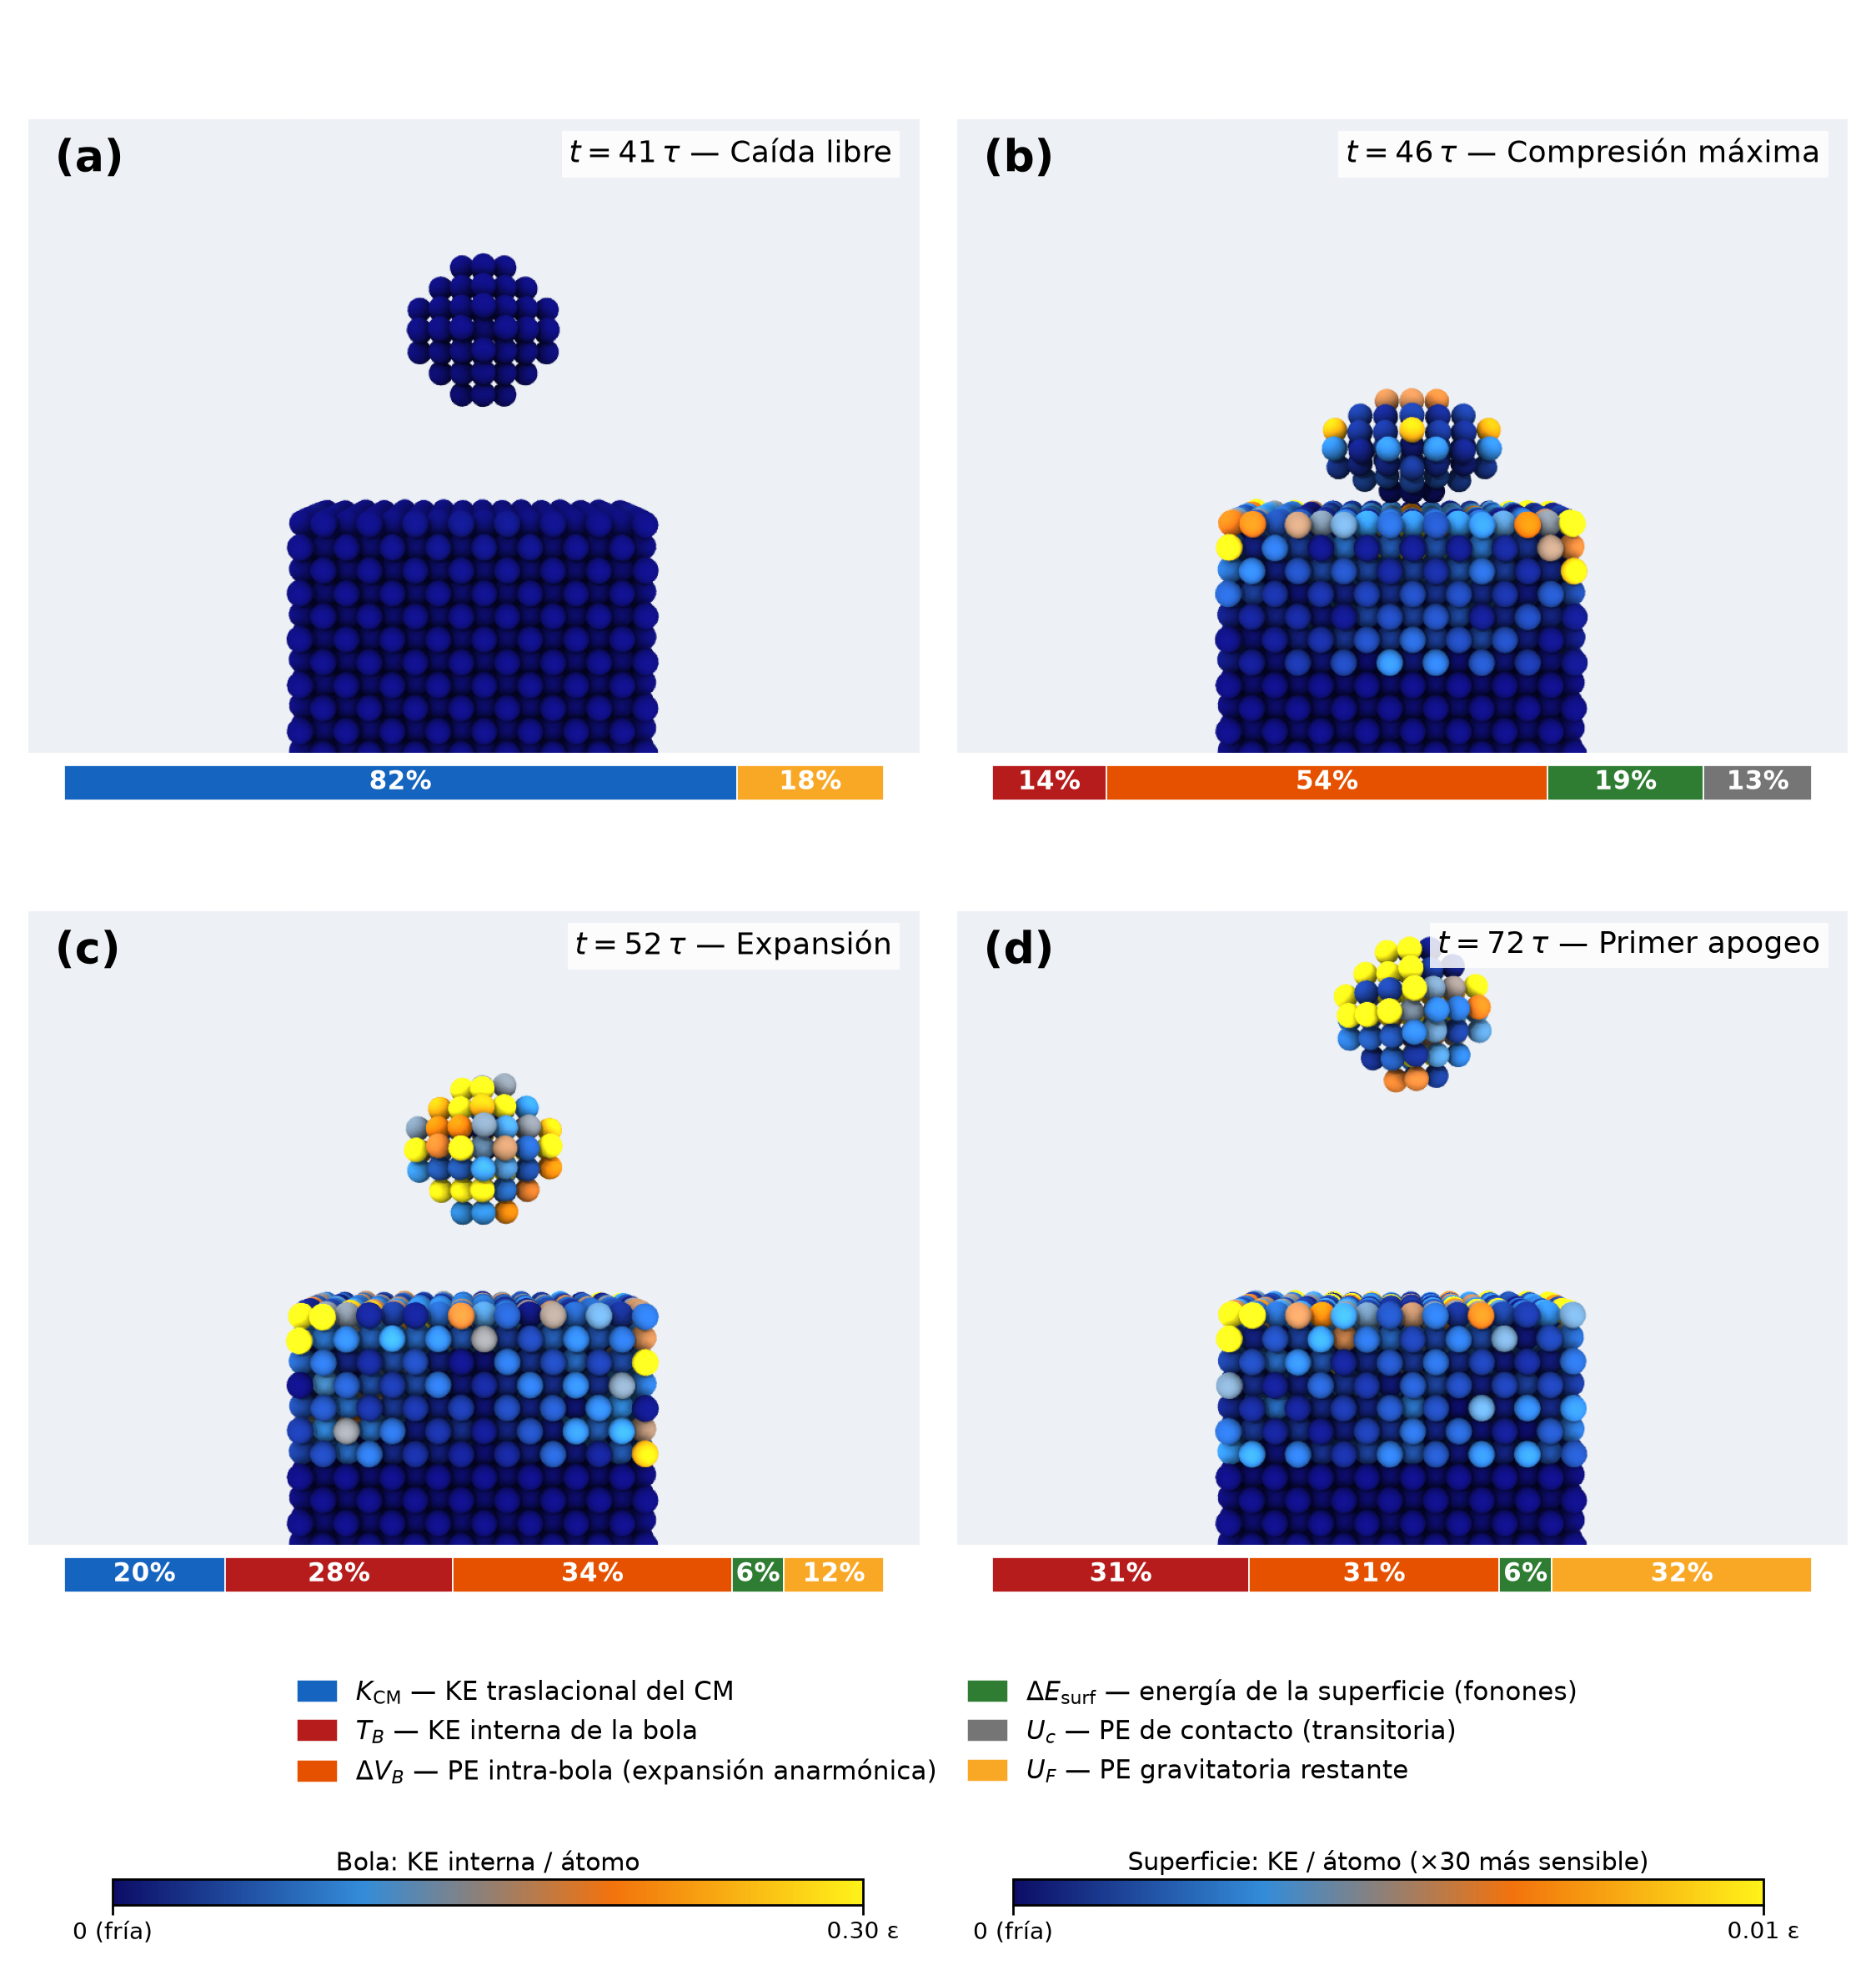
\includegraphics[width=\textwidth]{../figuras_rbef/fig_sequence.png}
    \caption{Cuatro instantes del primer rebote ($N=79$,
    $h_0=28.15\,\sigma$, $c_{ps}=0$): (a)~caída libre, (b)~compresión
    máxima, (c)~expansión post-impacto y (d)~primer apogeo. Los átomos de
    la bola se colorean por su KE interna (sin el movimiento del CM) y los
    de la superficie por su KE en una escala $\times30$ más sensible. La
    barra bajo cada panel es la partición instantánea de $E_0$; la energía
    de contacto $U_c$ (gris) solo existe durante la colisión.}
    \label{fig:secuencia}
\end{figure*}

La Tabla~\ref{tab:particion4} cuantifica la partición al primer apogeo
para seis alturas de caída. Tres observaciones para discutir con
estudiantes:

\begin{table*}[tp]
\centering
\small
\caption{Partición de la energía del primer rebote para $N=79$,
$c_{ps}=0$, $T=0$, promediada sobre 5 orientaciones iniciales del cúmulo
(media $\pm\sigma$; losa $8\times8\times6$). Por conservación,
$\alpha_{\rm cm}+\alpha_{T_B}+\alpha_{\Delta V_B}+\alpha_{\rm surf}=1$. La
dispersión entre orientaciones domina la incertidumbre; a alta energía
$\alpha_{\rm surf}$ está además subestimado $\sim0.06$ por tamaño finito de
losa (Sec.~\ref{sec:metodos}d).}
\label{tab:particion4}
\begin{tabular}{cccccc}
\toprule
$v_{\rm imp}$ ($\sigma/\tau$) & $e_1$ &
$\alpha_{\rm cm}$ & $\alpha_{T_B}$ & $\alpha_{\Delta V_B}$ &
$\alpha_{\rm surf}$ \\
\midrule
0.70 & $0.87\!\pm\!0.05$ & $0.76\!\pm\!0.08$ & $0.13\!\pm\!0.09$ & $0.04\!\pm\!0.02$ & $0.08\!\pm\!0.02$ \\
0.93 & $0.70\!\pm\!0.14$ & $0.51\!\pm\!0.17$ & $0.17\!\pm\!0.05$ & $0.21\!\pm\!0.17$ & $0.11\!\pm\!0.05$ \\
1.16 & $0.62\!\pm\!0.10$ & $0.40\!\pm\!0.12$ & $0.22\!\pm\!0.10$ & $0.24\!\pm\!0.10$ & $0.14\!\pm\!0.07$ \\
1.43 & $0.59\!\pm\!0.06$ & $0.35\!\pm\!0.06$ & $0.21\!\pm\!0.06$ & $0.26\!\pm\!0.09$ & $0.18\!\pm\!0.09$ \\
1.72 & $0.53\!\pm\!0.05$ & $0.28\!\pm\!0.05$ & $0.19\!\pm\!0.04$ & $0.31\!\pm\!0.05$ & $0.23\!\pm\!0.10$ \\
2.02 & $0.49\!\pm\!0.05$ & $0.24\!\pm\!0.05$ & $0.18\!\pm\!0.02$ & $0.31\!\pm\!0.05$ & $0.27\!\pm\!0.10$ \\
\bottomrule
\end{tabular}
\end{table*}

\textbf{Primero}, el rebote lento ($v_{\rm imp}=0.68\,\sigma/\tau$) es
casi elástico: el 85\% de la energía vuelve al CM. Apenas la velocidad de
impacto supera $\sim0.9\,\sigma/\tau$, la fracción cinética interna salta
a un \emph{plateau} $\alpha_{T_B}\approx0.21$--$0.24$ que se mantiene
hasta la máxima velocidad estudiada.

\textbf{Segundo}, existe un canal sin análogo macroscópico: la
\emph{expansión anarmónica} $\alpha_{\Delta V_B}$. Al comprimirse y
recalentarse, la bola queda vibrando alrededor de un estado expandido
(el potencial de la ecuación~(\ref{eq:lj}) es más blando hacia afuera que
hacia adentro), y esa energía potencial ``viaja'' con la bola. Es
comparable al canal cinético: $\alpha_{\Delta V_B}\approx0.21$--$0.33$.
En conjunto, la bola retiene como energía interna
$\alpha_{\rm bola}=\alpha_{T_B}+\alpha_{\Delta V_B}\approx0.4$--$0.6$ de
$E_0$.

\textbf{Tercero}, el piso se lleva poco:
$\alpha_{\rm surf}\approx0.08$--$0.27$ (con una corrección de tamaño finito
de losa, Sec.~\ref{sec:metodos}d). La intuición macroscópica ---``la
energía se disipa en el suelo''--- falla a esta escala: la respuesta
correcta a ``¿a dónde se fue la energía?'' es, en su mayor parte,
\emph{a la propia pelota}. Este desglose complementa el análisis
de~\cite{Gutierrez2012}, que describió el balance \emph{durante} el
contacto, donde domina la energía de contacto $U_c$; esa energía es
transitoria y regresa mayoritariamente a la bola cuando esta se separa.

% =============================================================================
\section{Equipartición: el tamaño de la pelota importa}
\label{sec:equiparticion}
% =============================================================================

¿Por qué la bola retiene justamente esa fracción? Un argumento de física
estadística da la respuesta, siempre que se aplique a la cantidad correcta.
La energía que \emph{no} regresa al CM, $1-\alpha_{\rm cm}$, es la única que se
reparte entre modos internos de la bola y de la superficie; el canal del CM no
participa de ese reparto. La fracción de esa energía disipada que queda en la
bola,
\begin{equation}
    f_{\rm ball} \equiv
    \frac{\alpha_{\rm bola}}{\alpha_{\rm bola}+\alpha_{\rm surf}},
    \label{eq:fball}
\end{equation}
es lo que la equipartición entre los $3N-3$ modos internos de la bola y
$3N_c^{\rm ef}$ osciladores \emph{netos} de la superficie debe predecir:
\begin{equation}
    f_{\rm ball}(N) = \frac{3N-3}{3N-3+3N_c^{\rm ef}}.
    \label{eq:equiparticion}
\end{equation}
Corrimos las seis alturas para $N\in\{1,2,7,13,55,79,87\}$, promediando cada
punto sobre cinco orientaciones iniciales del cúmulo; la
Tabla~\ref{tab:sweep_N} da las fracciones del plateau con su dispersión.

\begin{table*}[tp]
\centering
\small
\caption{Fracciones del primer rebote en el plateau
($1.1<v_{\rm imp}\lesssim1.7\,\sigma/\tau$), media $\pm\sigma$ sobre
orientaciones, vs $N$. Las dos últimas columnas son $N_c$ \emph{medido} en el
dump (huella geométrica y número de participación de la KE de superficie, a
$v_{\rm imp}\approx1.47$); no son ajustes.}
\label{tab:sweep_N}
\begin{tabular}{ccccccc}
\toprule
$N$ & $\alpha_{T_B}$ & $\alpha_{\rm bola}$ & $\alpha_{\rm surf}$ &
$f_{\rm ball}$ & $N_c^{\rm geom}$ & $N_c^{\rm part}$ \\
\midrule
 1  & $0.00$          & $0.00$          & $0.14\!\pm\!0.06$ & ---            & --- & --- \\
 2  & $0.09\!\pm\!0.11$ & $0.15\!\pm\!0.15$ & $0.21\!\pm\!0.09$ & $0.34\!\pm\!0.29$ & --- & --- \\
 7  & $0.24\!\pm\!0.15$ & $0.36\!\pm\!0.19$ & $0.23\!\pm\!0.06$ & $0.55\!\pm\!0.23$ & 47 & 284 \\
13$^a$ & $0.09\!\pm\!0.05$ & $0.21\!\pm\!0.12$ & $0.29\!\pm\!0.06$ & $0.38\!\pm\!0.13$ & 43 & 318 \\
55  & $0.14\!\pm\!0.07$ & $0.32\!\pm\!0.16$ & $0.27\!\pm\!0.05$ & $0.49\!\pm\!0.18$ & 67 & 341 \\
79  & $0.20\!\pm\!0.06$ & $0.48\!\pm\!0.13$ & $0.20\!\pm\!0.10$ & $0.70\!\pm\!0.14$ & 65 & 414 \\
87  & $0.24\!\pm\!0.04$ & $0.56\!\pm\!0.07$ & $0.17\!\pm\!0.08$ & $0.77\!\pm\!0.09$ & 93 & 397 \\
\bottomrule
\end{tabular}\\
\footnotesize $^a$ $N=13$ no alcanza el plateau en el rango estudiado
(ver texto).
\end{table*}

En vez de dejar $N_c$ como parámetro de ajuste, lo \emph{medimos} en la
simulación con dos estimadores sin parámetros libres, evaluados en la
compresión máxima: la huella geométrica $N_c^{\rm geom}$ (átomos de superficie
a $<r_c$ de algún átomo de la bola) y el número de participación de la energía
cinética de superficie, $N_c^{\rm part}=(\sum_i K_i)^2/\sum_i K_i^2$
(cuántos átomos comparten esa energía). La Figura~\ref{fig:sweep_N}(a) muestra
que aparecen \emph{tres escalas} bien separadas,
\begin{equation}
    N_c^{\rm ef}\approx25 \;\ll\; N_c^{\rm geom}\approx45\text{--}90
    \;\ll\; N_c^{\rm part}\approx300\text{--}410,
    \label{eq:escalas}
\end{equation}
donde $N_c^{\rm ef}$ es la capacidad \emph{neta} que se obtiene invirtiendo la
ecuación~(\ref{eq:equiparticion}). La lectura física resuelve la aparente
paradoja: cientos de átomos de la superficie se mueven \emph{transitoriamente}
durante el contacto ($N_c^{\rm part}$), pero la superficie es casi elástica y
\emph{devuelve} la mayor parte de esa energía cuando la bola despega; el sumidero
neto equivale a solo $\sim25$ osciladores. (El valor $N_c\approx290$ que
usábamos antes coincidía por accidente con $N_c^{\rm part}$: era el número
correcto en el balance energético equivocado.)

\begin{figure*}[tp]
    \centering
    \includegraphics[width=0.9\textwidth]{../figuras_rbef/fig_Nc_escalas.pdf}
    \caption{(a)~Las tres escalas de $N_c$ vs $N$: participación de la KE de
    superficie $N_c^{\rm part}$ y huella geométrica $N_c^{\rm geom}$
    \emph{medidas} en el dump, y capacidad neta $N_c^{\rm ef}\approx25$ (banda
    gris) obtenida de la partición; la recta punteada $N_c=N$ es la hipótesis
    previa, ahora descartada. (b)~Fracción de la energía disipada retenida por
    la bola, $f_{\rm ball}(N)$, con barras de error sobre orientaciones y el
    ajuste de la ecuación~(\ref{eq:equiparticion}) con
    $N_c^{\rm ef}=25\pm8$; tiende a $1$, no a $1/2$ (punteada).}
    \label{fig:sweep_N}
\end{figure*}

Ajustando la ecuación~(\ref{eq:equiparticion}) a $f_{\rm ball}(N)$ con
$N_c^{\rm ef}$ constante (excluyendo los dímeros, sin huella real) se obtiene
$N_c^{\rm ef}=25\pm8$: la capacidad neta de la superficie es pequeña y
prácticamente independiente de $N$ (Figura~\ref{fig:sweep_N}b). La consecuencia
reemplaza al límite $1/2$ que reportábamos antes:
\begin{equation}
    f_{\rm ball} \xrightarrow{N\to\infty} 1,
    \label{eq:limite}
\end{equation}
una pelota nanométrica grande, fría y sin adhesión retiene \emph{casi toda} la
energía que no devuelve al CM, porque sus $3N-3$ modos internos superan de largo
la capacidad fija $\sim3N_c^{\rm ef}$ de la superficie. El límite $1/2$ del
borrador anterior provenía de suponer $N_c=N$ (un oscilador de superficie por
átomo de la bola), hipótesis que tanto la medición directa
(ecuación~(\ref{eq:escalas})) como el análisis sobre la energía disipada
descartan.

El caso $N=13$ queda fuera de la tendencia: una sola capa FCC es demasiado
rígida para termalizar en el tiempo de contacto. Esa excepción es en sí misma
una lección: la equipartición requiere que el sistema \emph{alcance} a explorar
sus modos, y un cúmulo pequeño y rígido se comporta como molécula, no como
sólido.

\textbf{¿Sigue siendo sólida la bola?} El conteo de $3N-3$ modos supone una
bola sólida. Medimos su temperatura interna efectiva
$T_{\rm ef}=2T_B/(3N-3)$ en el apogeo y su estructura $g(r)$
(Figura~\ref{fig:fusion}). Para $N=79$, $T_{\rm ef}$ crece de $0.003$ a $0.28$
entre $v_{\rm imp}=0.68$ y $2.0\,\sigma/\tau$; comparado con la fusión de un
cúmulo LJ de $\sim80$ átomos ($T^*\approx0.30$--$0.35$), la bola permanece
sólida hasta $v_{\rm imp}\approx1.7$ (picos FCC nítidos, contraste
pico/valle $\approx11$) y solo en el extremo superior ($v\approx2$) se funde
(estructura colapsada, contraste $\approx2$). Por eso restringimos el plateau y
el conteo de modos de sólido a $v_{\rm imp}\lesssim1.7\,\sigma/\tau$; el punto
de $v\approx2$ pertenece ya al régimen de fusión de~\cite{Gutierrez2012}.

\begin{figure*}[tp]
    \centering
    \includegraphics[width=0.85\textwidth]{../figuras_rbef/fig_fusion_gr.pdf}
    \caption{Estructura de la bola $g(r)$ a $t=0$ (FCC, azul) y en el primer
    apogeo (rojo), para $N=79$. (a)~A $v_{\rm imp}=1.47$ los picos FCC
    (líneas punteadas) sobreviven: la bola sigue sólida. (b)~A
    $v_{\rm imp}=2.03$ los picos se funden: la bola se ha desordenado. Esto
    delimita el rango de validez del conteo de modos de sólido.}
    \label{fig:fusion}
\end{figure*}

% =============================================================================
\section{Rebotes sucesivos: una predicción y su límite}
\label{sec:hstar}
% =============================================================================

El plateau $\alpha_{T_B}\approx0.22$ sugiere una escala de altura para el
primer rebote: si $\alpha_{\rm cm}\approx\alpha_{T_B}$, entonces
\begin{equation}
    h_1 \approx h^* = \frac{T_B^{(1)}}{Mg}.
    \label{eq:hstar}
\end{equation}
Una simulación larga ($5000\,\tau$, $N=79$, $h_0=28.15\,\sigma$) permite
poner a prueba la ecuación~(\ref{eq:hstar}) rebote a rebote
(Figura~\ref{fig:largo}). Para el primer rebote funciona muy bien
($h_1/h^*=0.96$), pero la razón $h_n/h^*_n$ cae monótonamente en los
rebotes siguientes: la altura decae geométricamente mientras la energía
interna, ya depositada, decrece mucho más despacio. Tras 23 rebotes
($t\approx660\,\tau$) la bola queda atrapada sobre la superficie,
vibrando con $h_n\lesssim1\,\sigma$: el análogo nanométrico del final del
rebote de cualquier pelota real. (El posterior ``colapso'' de la bola a
través de la red, en $t\approx713\,\tau$, es un artefacto del potencial
puramente repulsivo, que no tiene barrera lateral; detectarlo y explicarlo
es otro buen ejercicio de análisis crítico de simulaciones.)

\begin{figure*}[tp]
    \centering
    \includegraphics[width=\textwidth]{../figuras_rbef/fig_paso_B_convergencia.pdf}
    \caption{Simulación larga ($5000\,\tau$, $N=79$,
    $h_0=28.15\,\sigma$). (a)~Trayectoria del CM; la línea roja marca el
    colapso a través de la red (artefacto del caso puramente repulsivo).
    (b)~Alturas de apogeo $h_n$ y predicción $h^*_n=T_B^{(n)}/(Mg)$.
    (c)~Razón $h_n/h^*_n$: solo el primer rebote se aproxima a la unidad.}
    \label{fig:largo}
\end{figure*}

% =============================================================================
\section{¿Y si la pelota es pegajosa? Adhesión}
\label{sec:adhesion}
% =============================================================================

Restaurando la atracción bola--superficie ($c_{ps}=1$ en la
ecuación~(\ref{eq:lj})), el experimento cambia cualitativamente: en los 24
casos estudiados ($N\in\{13,55,79,87\}$, seis alturas, $v_{\rm imp}$ hasta
$2\,\sigma/\tau$) la bola \emph{no rebota}: queda adherida al primer
contacto. La razón es un simple balance: la energía de adhesión medida,
$E_{\rm adh}\propto N^{0.73}$ (cercana al escalado del área de contacto,
$N^{2/3}$), supera con holgura a la energía que el CM logra retener tras
el impacto. Extrapolando ese balance, el umbral de rebote se ubicaría en
alturas de caída del orden de $h_0^*\sim10^2$--$10^3\,\sigma$ ---una
estimación de orden de magnitud, pues a esas velocidades la bola ya se
funde al impactar~\cite{Gutierrez2012}---, con la particularidad
contraintuitiva de que los cúmulos \emph{grandes} escapan más fácil
($h_0^*\propto N^{-0.27}$: la masa crece como $N$ pero la adhesión solo
como $N^{0.73}$). Este régimen conecta el experimento de aula con la
física de la deposición suave (\emph{soft landing}) de cúmulos sobre
superficies~\cite{Awasthi2007,Haberland1994}.

\begin{figure*}[tp]
    \centering
    \includegraphics[width=\textwidth]{../figuras_rbef/fig_paso_C_adhesion.pdf}
    \caption{Caso con adhesión ($c_{ps}=1$). (a)~Trayectorias del CM para
    $N=79$ y seis alturas: la bola pega al primer contacto en todos los
    casos. (b)~Umbral de rebote extrapolado $h_0^*(N)$ (estimación de
    orden de magnitud) y su escalado $\propto N^{-0.27}$.}
    \label{fig:adhesion}
\end{figure*}

% =============================================================================
\section{Actividades propuestas}
\label{sec:actividades}
% =============================================================================

El repositorio incluye todo lo necesario para reproducir el artículo.
Algunas actividades que hemos encontrado fructíferas, en orden de
dificultad creciente:

\begin{enumerate}
    \item \textbf{El COR no es constante.} Correr las seis alturas con
    $N=79$ y graficar $e_1$ vs $v_{\rm imp}$. Discutir por qué a bajas
    velocidades el rebote es casi elástico y contrastar con la hipótesis
    ``$e$ = constante del material'' de los textos de mecánica.

    \item \textbf{Cierre energético.} Medir los cuatro canales de las
    ecuaciones~(\ref{eq:acm})--(\ref{eq:avb}) y verificar
    $\sum\alpha_i=1$. Repetir con el potencial truncado sin desplazar y
    explicar el origen del error de cierre resultante.

    \item \textbf{Predecir antes de simular.} Con la
    ecuación~(\ref{eq:equiparticion}) y $N_c^{\rm ef}\approx25$, predecir
    $f_{\rm ball}$ para un tamaño no simulado (por ejemplo $N=43$,
    capa completa) y luego correr la simulación para contrastar. Medir además
    $N_c^{\rm part}$ en el dump con \texttt{medir\_Nc.py} y discutir por qué
    difiere de $N_c^{\rm ef}$.

    \item \textbf{El destino final.} Estimar con la
    ecuación~(\ref{eq:hstar}) la altura del primer rebote y, con la
    serie geométrica de $e_1^{\rm ef}$, el tiempo total hasta el
    atrapamiento; comparar con la simulación larga.

    \item \textbf{Gravedad como perilla.} Repetir el experimento con
    $\gstar$ diez veces mayor y discutir qué cambia (velocidad de
    impacto, tiempo de vuelo) y qué no (la partición a igual
    $v_{\rm imp}$).
\end{enumerate}

% =============================================================================
\section{Comentarios finales}
\label{sec:conclusiones}
% =============================================================================

La pelota que rebota, uno de los sistemas más familiares de la física
introductoria, se convierte a escala nanométrica en un laboratorio
completo: la dinámica molecular permite abrir la caja negra del
coeficiente de restitución y mostrar, con contabilidad exacta, que la
energía ``perdida'' se reparte en cuatro canales bien definidos
---y que la mayor parte queda dentro de la propia pelota, no en el piso.
El escalado con el tamaño conecta el resultado con el teorema de
equipartición: aplicado a la energía disipada, y con $N_c$ medido
directamente en la simulación en lugar de ajustado, predice que la fracción
retenida por la bola tiende a $1$ ---no a $1/2$--- para bolas grandes
(ecuaciones~(\ref{eq:equiparticion}) y~(\ref{eq:limite})). La lección
metodológica es doble: promediar sobre orientaciones es imprescindible para
separar señal de ruido, y un mismo símbolo ($N_c$) puede esconder tres
cantidades físicas distintas si no se lo mide. La simulación larga enseña la
diferencia entre una escala útil y un atractor; y el caso con adhesión abre la
puerta a la física de deposición de nanocúmulos. El costo computacional es el
de un computador personal y las herramientas son gratuitas: el experimento
completo cabe en un curso de física computacional, de física estadística o en
un trabajo de titulación.

Como extensiones naturales quedan la temperatura inicial finita, la medición
del momento angular post-rebote, la convergencia sistemática de
$\alpha_{\rm surf}$ con el tamaño de la losa, y los tamaños intermedios $N=19$
y $43$ para poblar la transición molécula--sólido entre $N=13$ y $N=55$.

% =============================================================================
\section*{Agradecimientos}
% =============================================================================

Los autores agradecen al programa de Magíster del Instituto de Matemáticas
de la PUCV por el apoyo académico. Las simulaciones se realizaron con
\lammps{}~\cite{Thompson2022}. El código fuente y los datos están
disponibles en \url{https://github.com/fwasaff/inelastic-rebound-md}.

% =============================================================================
\begin{thebibliography}{99}

\bibitem{Cross1999}
R. Cross, Am. J. Phys. \textbf{67}, 222 (1999).

\bibitem{Aguiar2003}
C.E. Aguiar y F. Laudares, Am. J. Phys. \textbf{71}, 499 (2003).

\bibitem{AllenTildesley}
M.P. Allen y D.J. Tildesley, \textit{Computer Simulation of Liquids}
(Oxford University Press, Oxford, 1987).

\bibitem{FrenkelSmit}
D. Frenkel y B. Smit, \textit{Understanding Molecular Simulation: From
Algorithms to Applications} (Academic Press, San Diego, 2002), 2.ª ed.

\bibitem{Gutierrez2012}
G. Gutiérrez, S. Davis, C. Loyola, J. Peralta, F. González, Y. Navarrete
y F. González-Wasaff, in \textit{Molecular Dynamics -- Theoretical
Developments and Applications in Nanotechnology and Energy}, editado por
L. Wang (InTech, Rijeka, 2012).

\bibitem{Thompson2022}
A.P. Thompson, H.M. Aktulga, R. Berger, D.S. Bolintineanu, W.M. Brown,
P.S. Crozier, P.J. in 't Veld, A. Kohlmeyer, S.G. Moore, T.D. Nguyen,
R. Shan, M.J. Stevens, J. Tranchida, C. Trott y S.J. Plimpton,
Comput. Phys. Commun. \textbf{271}, 108171 (2022).

\bibitem{Awasthi2007}
A. Awasthi, S.C. Hendy, P. Zoontjens y S.A. Brown,
Phys. Rev. B \textbf{76}, 115437 (2007).

\bibitem{Haberland1994}
H. Haberland, M. Mall, M. Moseler, Y. Qiang, T. Reiners y Y. Thurner,
J. Vac. Sci. Technol. A \textbf{12}, 2925 (1994).

\end{thebibliography}

\end{document}
